\section{Uvod}
U ovom radu je na DE1-SoC razvojnom sistemu implementiran jednostavan hardver u FPGA, portovan je Linuks operativni sistem i napisan je drajver za pristup registrima i prihvatanje prekida iz FPGA.

\subsection{Sistemi na čipu sa FPGA}
Sa sve većim mogućnostima namenskih sistema došlo je do popularizacije sistema na čipovima (SoC - \textit{System on Chip}) koji integrišu mikroprocesore sa više jezgara, memorije na čipu, mnogobrojne periferije i transivere, kao i FPGA (\textit{Field Programmable Gate Array}).

Ova tehnologija daje dizajneru sistema veliku slobodu i mogućnosti, a zadršava se klasičan postupak projektovanja namenskih sistema. Uz to se ostvaruje veća integracija, manja potrošnja, manja površina štampane ploče (PCB - \textit{Printed Circuit Board}) i veći protok podataka između procesora i FPGA dela. 

Uobičajena primena ovih sistema je implementacija specifičnih akceleratora koji ubrzavaju izvršavanje algoritama i implementacija specifičnih programabilnih interfejsa ka spoljnom svetu. Sve zrelije tehnologije kao što su OpenCL, Vivado HLS, Matlab HDL Coder omogućavaju kompatibilnost dizajna softvera na visokom nivou i implementiranog hardvera na niskom nivou.

SoC FPGA sistemi najčešće sadrže ARM mikroprocesor. Aplikacije na mikroprocesoru bez operativnog sistema (\textit{baremetal application}) nude jednostavno pisanje koda i uštedu na resursima. Za kompleksnije aplikacije koriste se operativni sistemi (OS) i time se olakšava integrisanje mrežnih protokola, rad sa multimedijalnim sadržajima, kriptografskim bibliotekama kao i mnoge druge mogućnosti koje su dostupne kao \textit{open-source} softver. Kada je potrebno garantovati reakciju u određenom vremenu na neki spoljni događaj veliki operativni sistemi nisu dobro rešenje i koriste operativni sistemi u realnom vremenu (RTOS - \textit{Real time operating system}).

Hardver u FPGA se projektuje upotrebom nekog od dva popularna jezika za opis hardvera - Verilog i VHDL (\textit{Very High Speed Integrated Circuit Hardwer Description Language}). Pored toga neophodni su softverski alati za specifični uređaj, koje obezbeđuje sam proizvođač uređaja. Dodatno ovi alati olakšavaju dizajn upotrebom IP(\textit{Intelectual Property}) blokova, generisanjem raznih izlaznih fajlova koji opisuju projektovani hardver na standardni način i koriste se prilikom razvoja softvera.

\subsection{Opis DE1-SoC}

U ovom radu korišćen je DE1-SoC razvojni sistem koji se vrlo često upotrebljava u edukativne svrhe. Razvojni sistem je zasnovan na čipu iz familije Cyclone V kompanije Intel (ranije Altera).

U nastavku su navedene samo osobine razvojnog sistema koje se tiču ovog rada, a detaljniji opis se moze pronaći u dokumentu zvaničnoj dokumentaciji proizvođača \cite{de1}
dodati referencu: 
\begin{itemize}
\item Sistem na čipu Cyclone V \texttt{5CSEMA5F31}
\item Memorija 1GB (2x256Mx16) DDR3 SDRAM povezana na HPS
\item Slot za Micro SD karticu povezan na HPS
\item UART na USB (USB Mini-B konektor)
\item 5 debaunsiranih tastera (FPGA x4, HPS x1)
\item 11 LE dioda (FPGA x10, HPS x 1)
\item 12V DC napajanje
\end{itemize}

\subsection{Opis Altera Cyclone 5}
Altera Cyclone V je SoC FPGA koji se sastoji od dva dela: procesorski deo (HPS -  \textit{Hard processor System}) i programabilni FGPA deo. HPS se sastoji od MPU (\textit{Microprocessor unit}) sa ARM Cortex-A9 MPCore sa dva jezgra i sledećih modula: kontroleri memorije, memorije, periferije, sistem interkonekcije, debug moduli, PLL moduli. FPGA deo se sastoji od sledećih delova: FPGA programabilna logika (\textit{look-up} tabele, RAM memorije, mnozači i rutiranje), kontrolni blok, PLL, kontroler memorije.

Svaki pin kućista je povezan na samo jedan od ova dva dela sistema, tako da HPS deo i FPGA deo ne mogu međusobno razmenjivati pinove.

\subsubsection{Konfigurisanje FPGA i pokretanje HPS}
Pri pokretanju HPS (\textit{boot}) može da učita program iz FPGA dela, iz eksterne \textit{flash} memorije ili preko JTAG. FPGA ima mogućnost da se konfiguriše softverski iz HPS korišćenjem periferije \textit{FPGA Manager} ili spoljnim programatorom. Kombinacije ovih mogucnosti daju nekoliko scenarija:
\begin{itemize}
\item nezavisno konfigurisanje FPGA i pokretanje HPS
\item konfigurisanje FPGA, zatim pokretanje HPS iz memorije koja se nalazi u FPGA
\item pokretanje HPS, zatim konfigurisanje FPGA iz HPS
\end{itemize}
DE1-SoC razvojni sistem dolazi sa integrisanim programatorom kojem se pristupa preko USB porta. Moguće je podesiti konfigurisanje FPGA spolja ili iz HPS upotrebom prekidača MSEL, dok se HPS uvek pokreće iz \textit{flash} memorije SD kartice.
(dodati tableu 3-2 iz de1soc user guide)

\subsubsection{HPS-FPGA interfejsi}
HPS-FPGA interfejsi su komunikacioni kanali između HPS i FPGA dela. U nastavku su nabrojani i opisani HPS-FPGA interfejsi:
\begin{itemize}
\item  FPGA-to-HPS bridge - magistrala visokih preformansi konfigurabilne sirine od 32,64 ili 128 bita. Na ovoj magistrali je FPGA master. Ovaj interfejs otkriva FPGA masterima ceo adresni prostor HPS dela.
\item HPS-to-FPGA bridge - magistrala visokih preformansi konfigurabilne sirine od 32,64 ili 128 bita. Na ovoj magistrali je HPS master a u FPGA se nalazi slave.
\item Lightweight HPS-to-FPGA - magistrala sirine 32 bita. HPS je master na ovoj magistrali. Ovaj interfejs manjeg protoka je namenjen za pristup statusnim i kontrolnim registrima periferijama implementiranim u FPGA delu.
\item FPGA manager - HPS periferja koja komunicira sa FPGA delom prilikom konfiguracije ili pokretanja (boot)
\item Prekidi - mogucnost povezivanja prekida iz FPGA na HPS kontroler prekida
\item HPS debug interfejs - omogućava da se debug mogućnosti prošire i na FPGA deo
\end{itemize}

Interfejsi koji su produžetak AXI magistrale na FPGA deo su FPGA-to-HPS bridge, HPS-to-FPGA bridge i Lightweight HPS-to-FPGA. Za povezivanje na ovu magistralu sa strane FPGA koristi se Avalon magistrala, stoga je neophodan AXI-Avalon bridge.

\subsubsection{Proces pokretanja HPS (boot)}
Pokretanje HPS je proces koji se obavlja u više koraka. Nakon izvršavanja svakog koraka se učitava i pokreće sledeći. Ovo je proces je sličan kod svih ARM procesora, a u nastavku je ukratko opisan za konkretnu platformu.

\begin{figure}[h!]
\centering
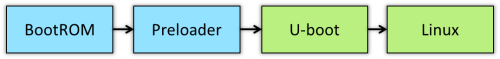
\includegraphics[scale=1.]{img/gsrd-boot.png}
\caption{Tok pokretana sistema}
\label{slika1:gsrd}
\end{figure}

Pri izlazu iz reset stanja procesor počinje izvrsavanje sa reset vektora iz memorije na čipu. Na adresi reset vektora je upisan Boot ROM progtam. Ovo je prvi korak u pokretanju HPS. \textit{Boot ROM} izvršava osnovna podešavanja procesora i dohvata \textit{preloader} iz NOR \textit{flash} memorije, NAND \textit{flash} memorije ili SD/MMC \textit{flash} memorije. Očitavaju se BSEL pinovi na osnovu kojih se određuje gde je smešten \textit{preloader}, zatim se inicijalizuje taj interfejs i učitava i pokreće \textit{preloader}. \textit{Boot ROM} softver proizvođača i ne može se menjati. 

\textit{Preloader} je prvi korak u pokretanju koji može da se konfiguriše. \textit{Preloader} obično izvršava inicijalizaciju SDRAM, dodatna podešavanja sitema, inicijalizaciju \textit{flash} kontrolera koji sadrži sledeći program (NAND, SD/MMC, QSPI) i zatim učitavanje programa u RAM memoriju i pokretanje.

Softver koji sledi nakon \textit{preloader}-a može biti \textit{baremetal} aplikacija ili \textit{bootloader}. \textit{Preloader} i svi prethodni programi se izvršavaju na prvom jezgru procesora dok je drugo u reset stanju. Naredni koraci mogu inicijalizovati drugo jezgro.

\textit{Bootloader} ima zadatak da podesi promenljive okruženja operativnog sistema, dohvati fajlove za pokretanje operativnog sistema (sa \textit{flash} memorije, putem \textit{Etherneta} preko TFTP protokola ili USB), konfigurise FPGA pruži konzolu za korisničke operacije. Neki od populatnih \textit{open-source} \textit{bootloader}-a su U-Boot i Barebox.

\subsection{Alati}
U nastavku će ukratko biti opisani korišćeni alati sa izdvojenim najvažnijim mogućnostima:
\begin{itemize}
\item Quartus Prime 18.0 - alat za razvoj hardvera na FPGA. Deo paketa je Platform Designer (ranije Qsys) koji u dizajn ukljucuje HPS, IP blokove i definiše povezanost ovih delova
\item \textit{Preloader Generator} (\texttt{bsp-editor} alat iz SoC EDS) - Generiše izvorni kod \textit{preloader}-a na osnovi izlaznih fajlova koji opisuju hardver
\item \textit{Device Tree Generator} (\texttt{sopc2dts} alat iz SoC EDS) - Generiše \textit{Device Tree} opis hardvera na osnovi izlaznih fajlova koji opisuju hardver
\item \textit{DE1-SoC Builder} - Generise prazan \textit{Quartus} projekat za DE1-SoC razvojni sistem
\item \textit{Linaro Toolchain} - koristi se za kompajliranje softvera
\end{itemize}

Na slici \ref{slika1:gsrd} je grafički prikazan tok projektovanja jednog SoCFPGA sistema.

\begin{figure}[h!]
\centering
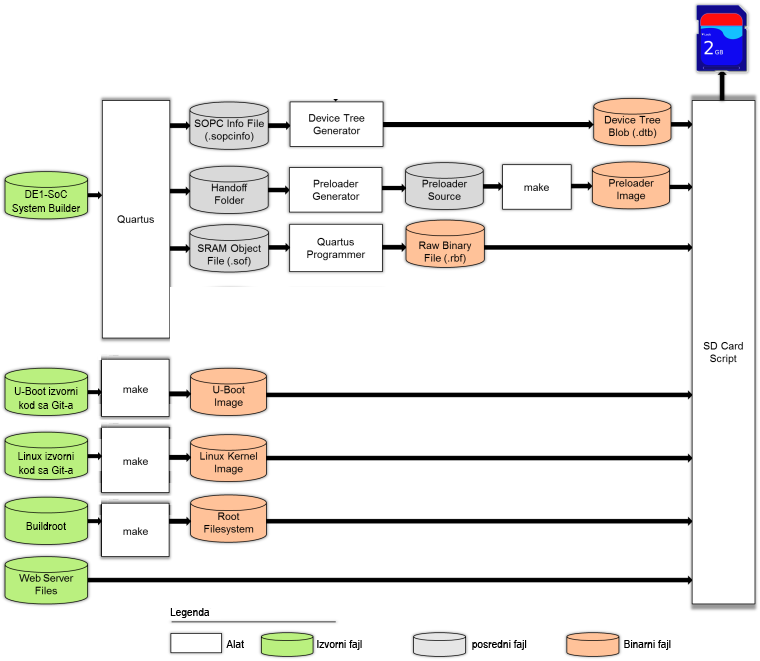
\includegraphics[scale=1.3]{img/gsrd-flow.png}
\caption{Tok projektovanja}
\label{slika1:gsrd}
\end{figure}

U nastavku su objašnjeni fajlovi koji se koriste pri projektovanju:
\begin{itemize}
\item \texttt{.qpf} - projektni fajl za Quartus. Ovaj fajl generiše DE1-SoC Builder
\item \texttt{.qsf} - skripta za podešavanje pinova. Ovaj fajl generiše DE1-SoC Builder
\item \texttt{.sdc} - skripta za podešavanje takta. Ovaj fajl generiše DE1-SoC Builder
\item \texttt{.v} - Verilog HDL izvorni kod
\item \texttt{.vhd} - VHDL izvorni kod
\item \texttt{.sof} -  SDRAM Object File - fajl za programiranje FPGA.  Ovaj fajl generiše Quartus pri kompajliranju dizajna
\item \texttt{.rbf} - \textit{Raw Binary File} - fajl za programiranje FPGA. Ovaj fajl se dobija konverzijom \texttt{.sof} alatom \texttt{quartus\_cpf}
\item \texttt{.dts} - \textit{Device Tree Source} - opis hardvera za Linuks kernel
\item \texttt{.dtb} - \textit{Device Tree Blob} - binarni fajl, kompajlirani opis hardvera za Linuks kernel
\item \texttt{.sopcinfo} - sadrži opis hardvera na osnovu kog se generišu drugi fajlovi. Ovaj fajl generiše \textit{Platform Designer}
\item \texttt{.c} - izvorni kod u jeziku C
\item \texttt{Makefile} - sadrži set direktiva za \texttt{make buld system}
\end{itemize} 
\pagebreak
\section{Opis projektovanog sistema}

U ovom radu je implementiran jednostavan sistem koji demonstira osnovne mogucnosti u dizajniranju sistema na SoC FPGA. Na slici \ref{slika:q3} je prikazan realizovani sistem (dodati novu sliku?)

\begin{figure}[h!]
\centering
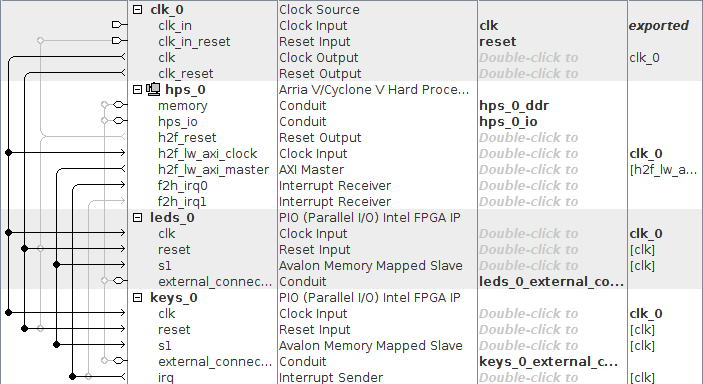
\includegraphics[scale=0.9]{img/quartus3.png}
\caption{Blok šema sistema}
\label{slika:q3}
\end{figure}

\subsection{Memorijski mapiran interfejs ka LE diodama i tasterima u FPGA}
Za projektovanje hardvera u FPGA koristi se PIO (\textit{Parallel Input/Output}) Intel FPGA IP blok. Ovo je jedan od mnogih dostupnih Intelovih IP blokova sa standardizovanim \textit{Avalon Memory Mapped Slave} interfejsom. HPS sistem pristupa registrima periferija implementiranih u FPGA (\textit{soft cores}) preko standardne AXI magistrale. Između Avalon i AXI magistrale nalazi se automatski generisani \textit{bridge}.

PIO Intel FPGA IP blok ima mogućnost da se konfiguriše kao ulazni, izlazni ili bidirekcioni. Takođe postoji mogućnost generisanja prekida na uzlaznu, silazni ili obe ivice ulaznog signala kao i mogućnost generisanja prekida na osnovu nivoa ulaznog signala. Dostupna su podešavanja za širinu paralelnog porta.

U tabeli ref su opisani registri PIO Intel FPGA IP bloka.

PIO Intel FPGA IP je u ovom radu iskorišćen za jednostavnu demonstraciju tako što je povezan na pinove Cyclone V sistema na čipu koji su na DE1-SoC razvojnom sistemu povezani na LE diode i tastere. U slučaju konkretne primene na rešavanje nekog problema, PIO Intel FPGA IP pruža jednostavan memorijski mapiran interfejs i mogućnost slanja prekida iz FPGA dela. Ova mogućnost korisna je u slučaju kada je za rešeavanje datog problema pogodno implementirati prizvoljno rešenje u pogramabilnoj logici. Ovaj pristup pruža slobodu projektovanja sistema u programabilnoj logici, a sa druge strane se zadržava standardizovani interfejs prema kompleksnom sistemu procesora. Na primer, izlazi PIO Intel FPGA IP registara mogu se koristiti kao konfiguracioni registri koji će upravljati korisničkom logikom, kao način da se pogramabilnoj logici dostave podaci koji će zatim biti obrađeni i vraćeni nazad. Mogućnost slanja prekida koristna je kada se PIO Intel FPGA IP koristi za posmartanje toka izvršavanja algoritma u programabilnoj logici - na promenu nekog signala se generiše prekid i opciono zatim očitava iz statusnog regisra potrebna informacija koja oslikava stanje sistema. Takođe, prekid se može koristiti za sinhronizaciju toka podataka pri obradi podataka u FPGA tj. kao vid da se mikroprocesoru javi da su podaci spremni za čitanje. Rezultati rešavanja problema u FPGA se mogu učinti dostupnim spoljnom svetu preko nekog od mnogih standardnih interfejsa (USB, Ethernet, UART, ...) i to vrlo jednostavnim postupcima u okviru operativnog sitema na HPS delu.

U ovom projektu u FPGA delu su postavljena dva PIO (\textit{Parallel Input/Output}) Intel FPGA IP bloka. PIO IP blok \texttt{leds\_0} je izlazni i koristi se za kontrolisanje LE dioda. PIO IP blok \texttt{keys\_0} je ulazni i koristi se za očitavanje tastera. PIO IP blok \texttt{keys\_0} takođe šalje prekidni zahtev HPS-u na svaku uzlaznu i silaznu ivicu.

\subsection{Preloader}
Pri pokretanju HPS sistema koristi se \textit{preloader} generisan Alterinim alatima. Za generisanje \textit{preloader}-a neophodni su fajlovi za opis sistema koje generiše Platform Designer. Program za generisanje \textit{Preloader Generator} je deo Alterinog SOC EDS(\textit{Embedded Development Suite}) paketa alata. U grafičkom meniju se odabira folder u kojem se nalazi Platform Designer projekat sistema za koji se generiše \textit{preloader}. Ovako generisani \textit{preloader} je zasnovan na SPL (\textit{Secondary Program Loader}) \textit{framework}-u koji je deo U-Boot projekta. Ovo ima pozitivnu posledicu da \textit{preloader} i U-Boot dele dosta izvornog koda, kao što je mnoštvo pouzdanih drajvera.

Standardna uloga \textit{preloader}-a za Cyclone V sistem na čipu je da:
\begin{itemize}
\item inicijalizacije SDRAM interfejsa uključujići kalibraciju SDRAM PLL modula
\item dohvata \textit{bootloader} binarnog fajla sa \textit{flash} memorije (NAND, SD/MMC, NOR)
\item smešta binarni fajl \textit{bootloader}-a u SDRAM i prepušta tok izvršavanja
\item konfiguriše multipleksiranje pinova(podešavanja za konfiguraciju su dostupna u Platform Designeru)
\item konfiguriše PLL na osnovu korisničkih podešavanja dostupnih u \textit{preloader generator}-u
\item otpušta određene periferije iz stanja reseta (izbor periferija se konfiguriše u Platform Designer-u)
\item inicijalizuje \textit{flash} kontroler (bilo NAND, SD/MMC ili QSPI) na osnovu \textit{boot} prekidača
\end{itemize}

U ovom radu se \textit{preloader} koristi za učitavanje i pokretanje U-boot \textit{bootloader}-a. Izvršni fajl \textit{bootloader}-a se nalazi na SD kartici. DE1-SoC razvojni sistem je već podešen za pokretanje sistema sa SD kartice, pa je preostalo u \textit{preloader generator}-u uključiti podršku za FAT fajl sistem i definisati ime binarnog fajla \textit{bootloader}-a. Nakon konfigurisanja \textit{preloader}-a potrebno je kompajlirati izvšni fajl koji će se prebaciti na razvojni sistem. Kompajliranje se vrši jednostavnim pozivom \textit{make} naredbe koja pokreće skriptu za \textit{make build system} koja kao rezultat daje izvršni fajl.

Ovaj izvršni fajl je potrebno prebaciti na SD karticu na posebnu particiju. Prilikom particionisanja SD kartice neophodno je predvideti ovu particiju i podesiti njen tip na posebnu vrednost \texttt{a2}.

\subsection{Bootloader}
\textit{Open-source} projekat U-Boot (\textit{Universal Boot Loader}) je uobičajeni izbor \textit{bootloader}-a za namenske sisteme zasnovane na ARM, PowerPC, MIPS procesorima. U-Boot se u ovom radu koristi za programiranje FPGA i učitavanje operativnog sistema. Ovo se postiže zahvaljujući tome što U-Boot nudi korisniku komandnu liniju koja se jednostavno može koristiti za pisanje skripti za željeno ponašanje \textit{bootloader}-a.

U-Boot se preuzima u obliku izvornog koda sa \texttt{git}-a[ref na git]
https://github.com/u-boot/u-boot
"Das U-Boot" Source Tree
Kako U-Boot podržava različite arhitekture potrebno je izvršiti konfiguraciju softvera. Konfiguracija je dostupna kao gotova za mnoge razvojne sisteme. Izvorni kod se konfiguriše kroz Kbuild infrastrukturu koja je se takođe koristi za konfiguraciju Linuksa. Konfiguracija se pokreće pozivom \texttt{make menuconfig} iz komandne linije i pruža vrlo jednostavan grafički interfejs i veliku moć podešavanja.

Konfiguracija za DE1-SoC razvojni sistem je dostupna kao gotova, što znači da se lako dobija funkcionalno konfigurisan izvorni kod. Osim toga, ovom konfigracijom dostupne su komande programiranja FPGA dela preko \textit{FPGA Manager} periferije.

Nakon osnovnog konfigurisanja softvera potrebno je napisati skriptu za željeno ponašanje i konfigurisanje U-Boot da pri pokretanju izvrši tu skriptu. Kroz Kbuild sistem se menja vrednost promenljive \textit{bootcmd} koja sadrži komandu koja će biti izvršena odmah po pokretanju sistema ukoliko korisnik ne prekine ovaj proces. Promenljiva \textit{bootcmd} je podešena tako da se izvrši kratka skripta za učitavanje naredne korisničke skripte (podešena je komanda \textit{run callscript}). Dalje, u izvornom kodu je na mestu predviđenom za korisničke definicije definisana jednostavna skripta \textit{callscript} koja samo učitava narednu korisničku skriptu (nazvanu \textit{u-boot.scr}). Na ovaj način je ostavljena sloboda za izmenu skripte i time ponašanja \textit{bootloader}-a bez potrebe da se ponovo konfiguriše i kompajlira U-Boot.

Ovim je konfiguracija U-Boot \textit{bootloader}-a završena i zatim se vrši kompajliranje kako bi se dobio izvršni fajl. Za kompajliranje koristi se \textit{Linaro toolchain}.
\subsubsection{Skripta za U-Boot}
Skripta za U-Boot piše se kao tekstualni i svodi se na pozive U-Boot komandi i definisanje vrednosti promenljivih. U-Boot komande pružaju velike mogućnosti i razlišite načine pokretanja operativnog sistema. Uobičajene primene ovih U-boot su:
\begin{itemize}
\item podešavanje promenljivih okruženja operativnog sistema
\item dohvatanje binarnih fajlova za pokretanje operativnog sistema iz \textit{flash} memorije ili preko \textit{ethernet}-a pri čemu je omogućen pristup standardnim fajl sistemima kao i prenos preko mreže preko TFTP(\textit{Trivial File Transfer Protocol})
\item smeštanje binarnih fajlova za pokretanje sistema u SDRAM i prepuštanje toka izvršavanja
\item podešavanje \textit{boot} argumenata koja se koriste za podešavanje kernela operativnog sistema
\end{itemize}

Nakon pisanja skripte potrebno je \textit{mkimage} alatom dodati odgovarajući U-Boot heder. Fajl koji se dobija je potrebno prebaciti na SD karicu na FAT particiju. U-Boot je već konfigurisan tako da učita i izvrši ovu skriptu, kao što je opisano ranije.

U ovom radu skripta je napisana tako da programira FPGA i pokrene Linuks operativni sistem. Fajlovi koje U-Boot čita pri izvršavanju ove skripte su:
\begin{itemize}
\item \texttt{socfpga.rbf} - binarni za konfiguraciju FPGA
\item \texttt{socfpga.dtb} - binarni fajl koji opisuje hardversku platofrmu i proslešuje se Linuks kernelu
\item \texttt{zImage} - kompajlirani kernel
\end{itemize}

U skripti se podešava vrednost promenljive \texttt{bootargs} koja definiše argumente koji će biti prosleđeni kernelu pri pokretanju operativnog sistema. Ova promenljiva podešena je tako da definiše veličinu RAM memorije, parametre konzole za komunikaciju sa sistemom i određuje \texttt{ext3} particiju SD kartice kao \textit{root file system} Linuksa.

Nakon učitavanja ovih fajlova izvršavaju se sledeće važne komande:
\begin{itemize}
\item \texttt{fpgaload} - za programiranje FPGA
\item \texttt{bridge enable} - za inicijalizaciju AXI magistrale između FPGA dela i HPS dela
\item \texttt{bootz} - komanda za pokretanje pokretanje operativnog sistema pri čemu se kernelu prosleđuje \textit{Devie Tree Blob} i argumenti iz promenljive \texttt{bootargs}
\end{itemize}

\subsection{Device Tree}
\textit{Device Tree} ili skraćeno DT je struktura podataka koja opisuje hardver. Koristi se za identifikaciju platforme i podešavanja u toku izvršavanja kao što je vrednost argumenata pri pokretanju kernela (promenljiva \textit{bootargs} koja je pomenuta ranije). Izdvajanje detaljnih informacija o sistemu u poseban fajl je uvedeno iz potrebe da se standardizuje način pokretanja kernela i interfejs između \textit{bootloader}-a i kernela i omogući jednostavno dodavanje novih platofrmi. Tako na primer jednom kompajlirani kernel može da se koristi na različitim platformama. \textit{Device Tree Source} koji opisuje detalje hardvera se kompajlira alatom \textit{Device Tree Compiler} u binarni fajl \textit{Device Tree Blob}. \textit{Device Tree Blob} učitava \textit{bootloader} i prosleđuje kernelu.
\subsubsection{Struktura Device Tree}
\textit{Device Tree} struktura podataka je organizovana kao drvo tako da se sastoji od čvorova (\textit{node}). Svaki čvor u ovoj strukturi mora imati čvor koji se nalazi iznad njega u hijerarhiji (\textit{parent node}) osim korena stabla (\textit{root node}). Svaki čvor predstavlja jedan drajver ili modul i sadrži opis osobina. Ukoliko postoje pravila za organizaciju informacija unutar čvora ona su opisana u \textit{bindings} delu u Linuks dokumentaciji[https://github.com/torvalds/linux/tree/master/Documentation/devicetree/bindings] \textit{Device Tree} ne mora da opiše svaki deo hardvera, a čvorovi koji su uobičajeni opisuju:
\begin{itemize}
\item procesori sistema (ovaj čvor je neophodan po specifikaciji)
\item memorije sistema (ovaj čvor je neophodan po specifikaciji)
\item specijalni konfiguracioni čvor za podešavanje argumemnata pri pokretanju kernela, podrazumevanih ulazno/izlaznih uređaja (ovaj čvor je neophodan po specifikaciji)
\item čvor koji opusje generalne osobine sistem na čipu (ovaj čvor je neophodan ukoliko je procesor u sistemu na čipu)
\item čvorovi koji opisuju magistrale sistema (ovaj čvor nije neophodan ali se preporučuje)
\end{itemize}

Neke od vaznih osobina u čvoru su:
\begin{itemize}
\item \texttt{compatible} - koristi se da označi kompatibilnost uređaja sa porodicom sličnih uređaja i za uparivanje drajvera i uređaja
\item \texttt{reg} - opisuje deo adresnog prostora u kom se nalazi uređaj kao par: početna adresa i dužina adresnog opsega
\item \texttt{\#address-cells} - određuje koliko 32-bitnih ćelija se koristi za opis početne adrese u \texttt{reg}
\item \texttt{\#size-cells} - određuje koliko 32-bitnih ćelija se koristi za opis dužine adresnog opsega u \texttt{reg} polju
\item \texttt{interrupts} - koristi se za uređaje koji generišu prekid i opisuje najčešće broj prekida i tip (nivo/ivica)
\item \texttt{interrupt-parent} - koristi se za uređaje koji generišu prekid i pokazuje na kontroler prekida kojem se šalje prekidni zahtev
\item \texttt{interrupt-controller} - \texttt{boolean} vrednost koja označava da li je uređaj kontroler prekida
\item \texttt{\#interrupt-cells} - određuje koliko 32-bitnih ćelija se koristi za opis \texttt{interrupts} polja u uređajima koji koriste kontroler prekida
\end{itemize}

U nastavku(premestiti u dodatak?) je na primeru dat pojednostavljeni \textit{Device Tree Source} koji opisuje DE1-SoC razvojni sistem. Na osnovu prethodnog teksta se lako može razumeti organizacija i sastav sistema. Dati primer je pojednostavljen tek toliko što su izostavljeni uređaji sistama na čipu čiji rad se ne izučava u ovom radu. Ceo \textit{Device Tree} je podeljen u nekoliko fajlova i može se pronaći u dodatku ovog rada i literaturi\cite{dts}. Iz priloženog koda se vidi da se sistem sastoji od:
\begin{itemize}
\item dva procesorska jezgra Cortex-A9
\item standardni ulazno/izlazni uređaj je serijski uređaj \texttt{serial0}
\item RAM memorija je kapaciteta 1GB
\item koristi se kontroler prekida  ARM \textit{Generic Interrupt Controller}
\item na memorijskoj adresu \texttt{0xff200000} koja odgovara početku adresnog prostora AXI magistrale koji izlazi prema FPGA se nalazi korisnički hardver koji se implementira u ovom radu i zauzima adresni opseg dužine 32 memorijske lokacije, prekidni zahtev je pod brojem 40 i ostljiv je na uzlaznu i silaznu ivicu
\item \texttt{serial0} je periferija \texttt{uart0} na naznačenoj adresi i sa naznačenim brojem prekida
\end{itemize}
\begin{lstlisting}[language=C]
/ {
	#address-cells = <1>;
	#size-cells = <1>;
	
	cpus {
		#address-cells = <1>;
		#size-cells = <0>;

		cpu0: cpu@0 {
			compatible = "arm,cortex-a9";
			device_type = "cpu";
			reg = <0>;
		};
		cpu1: cpu@1 {
			compatible = "arm,cortex-a9";
			device_type = "cpu";
			reg = <1>;
		};
	};
	
	chosen {
		bootargs = "earlyprintk";
		stdout-path = "serial0:115200n8";
	};

	memory@0 {
		name = "memory";
		device_type = "memory";
		reg = <0x0 0x40000000>; /* 1GB */
	};

	intc: intc@fffed000 {
		compatible = "arm,cortex-a9-gic";
		#interrupt-cells = <3>;
		interrupt-controller;
		reg = <0xfffed000 0x1000>,
		      <0xfffec100 0x100>;
	};
	soc {
		#address-cells = <1>;
		#size-cells = <1>;
		compatible = "simple-bus";
		device_type = "soc";
		interrupt-parent = <&intc>;
		ranges;
		
		lddipl0: lddipl@0xff200000 {
			compatible = "ld,dipl";
			reg = <0xff200000 0x00000020>;
			interrupts = <0 40 1>;
			
		uart0: serial0@ffc02000 {
			compatible = "snps,dw-apb-uart";
			reg = <0xffc02000 0x1000>;
			interrupts = <0 162 4>;
		};
\end{lstlisting}

Kada je \textit{Device Tree Source} napisan potrebno je smestiti \texttt{.dts} fajl u folder \texttt{arch/arm/boot/dts/}. Kompajliranje izovrnog opisa u binarni fajl \textit{Device Tree Blob} se ivršava komandom \texttt{make *.dtb} gde je potrebno upisati naziv fajla koji se kompajlira.

Potrebno je napomenuti da je u ovom radu modifikovan \textit{Device Tree} za razvojni sistem \textit{Cyclone V Develompent Kit} koji je veoma sličan DE1-SoC. Uvedene modifikacije se svode na isključivanje CAN uređaja koji Cyclone V \textit{Develompent Kit} ima a DE1-SoC nema. Zatim je dodat opis implementiranih PIO Intel FPGA IP u FPGA. Drugi način dobijanja \textit{Device Tree} koji nije zahtevao ručnu modifikaciju je korišćenje \textit{Device Tree Generator}-a koji je dostupan u okviru \textit{Altera Embedded Develompment Suite} paketa softverskih alata. Za ovaj način je testiranjem utvrđeno da postoji sledeći problem: drajver ne vidi uređaje koji pripadaju čvoru \texttt{bridge} koji opisuje adresni prostor između FPGA i HPS i samim tim i generisani hardver u FPGA. Najverovatniji razlog ovom problemu je različita verzija kernela od one za koju je alat namenjen, ali je u skladu sa edukativnim ciljem ovog rada izabran put ručnog pisanja \textit{Device Tree} umesto korišćenja generisanog.

\subsection{Linuks kernel}
Linuks kernel centralni deo operativnog sistema koji ima zadatak da upravlja resursima sistema i pruži interfejs prema hardveru. Linuks kernel je \textit{open-source} projekat koji održava i razvija veliki broj programera i kompanija. Izvorni kod je otvoren što omogućava prilagođavanje za različite platforme i privlači razvoj raznih kompatibilnih projekata. Ova osobina čini Linuks veoma popularnim u namenskim sistemima. Prednosti su portabilnost i hardverska porška koju pruža zajednica i proizvođači. Kernel je skalabilan pa se može konfigurisati za izvršavanje na super-računarima kao i na malim uređajima sa tek 4MB RAM memorije. Takođe, Linuks nudi gotove implementacije raznih delova sistema koji su potrebni za povezivanje i bezbednost.

Glavne uloge kernela su da upravlja harverskim resursima procesorom, memorijom i ulazno/izlaznim uređajima. Iz ugla razvoja softvera kenrel nudi standardizovani interfejs (API Application Programming Interface) koji je portabilan i nezavistan od arhitekture i specifičnog hardvera. Ovaj interfejs nudi korisne apstrakcije koje su prikazane na slici \ref{slika1:linux1}.\\
\begin{figure}[h!]
\centering
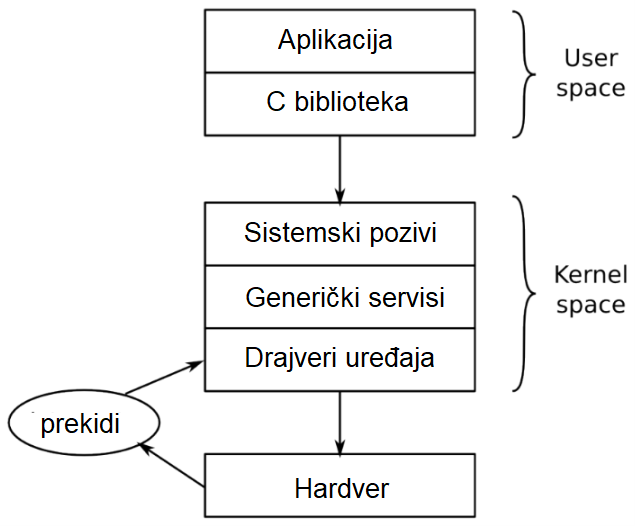
\includegraphics[scale=0.5]{img/linux1.png}
\caption{Organizacija linuksa}
\label{slika1:linux1}
\end{figure}
Korisničke aplikacije uglavnom pozivaju standardnu C biblioteku. C biblioteka se obraća kernelu preko sistemskih poziva, a implementacija sistemskih poziva je različita u zavisnosti od arhitekture sistema. Drajveri uređaja pružaju interfejs prema hardveru i biće detalnije objašnjeni kasnije.

Jedna od osnovnih odlika Linuks kernela je podela sistema na privilegovani \textit{kernel-space} deo i na neprivilegovani \textit{user-space} deo. U privilegovanom režimu kernel ima pristup zaštićenom delu memorije i slobodan pristup hardveru. \textit{User-space} je namenjen za aplikacije kojima je dozvoljen ograničen pristup određenim resursima. Međutim, jedna od korisnih mogućnosti za namenske sisteme dostupna u \textit{user-space}-u je pristup memorijskom prostoru u kojem se nalaze periferije. Ovo se postiže mapiranjem memorijskog prostora u virtuelnu adresu. Ovaj način pristupa registrima je zgodan jer je brz i jednostavan, a u nekim slučajevima je dovoljan za rešavanje datog problema \cite{mmap}. Veliki nedostatak ovog pristupa je što ne postoji način da se registruju prekidne rutine.

U ovom radu korišćena je verzija 4.6 Linuks kernela dostupna na \texttt{git} repozitorijumu kompanije Altera. Verzije kernela koje obezbeđuju proizvođači su modifikovane za podržane platforme tako što su dodate konfiguracije i drajveri. Veći proizvođači vremenom unete izmene unesu i u glavnu verziju kernela. U ovom radu je korišćena Alterina verzija jer se preporučuje prema zvaničnim uputstvima.

Po preuzimanju izvornog koda vrši se konfiguracija upotrebom podrazumevanog konfiguracionog fajla za Alterine sisteme na čipu. Konfiguracija se izvršava komandom \texttt{make socfpga\_defconfig}. Nakon toga se pokreće kompajliranje kernela komandom \texttt{make zImage}. U folder \texttt{arch/arm/boot} se nalazi izvršni fajl \texttt{zImage} koji je spreman za prebacivanje na SD karticu.
\subsection{Root fajl sistem}
\textit{Root} fajl sistem je neophodan deo operativnog sistema. \textit{Root} označaca koren fajl sistema i postavlja se na nekom fajl sistemu koji se nalazi na trajnoj memoriji. Struktura \textit{root} fajl sistema je uređena standardnom \cite{fhs} koji definiše strukturu i nazive fodlera kao i njihovu namenu. Neophodno je da sa na definisanim mestima u \textit{root} fajl sistemu nalaze sva potrebna podešavanja za ispravno pokretanje kernela, kao i korisničke aplikacije koje implementiraju veoma koriste funkcionalnosti sistema.

U nekim delovima \textit{root} fajl sistema se nalaze virtuelni fajl sistemi koji nude organizovanu reprezentaciju struktura podataka kernela. Neki od ovih virtuelnih fajl sistema nude korisne mogućnosti kao što je modifikacija parametara kernela. Za ovaj rad je važno pomenuti folder \texttt{dev} u kojem se nalaze svi uređaji na sistemu predstavljeni kao fajlovi i folder \texttt{sys} koji će detaljnije biti opisan kasije.

\textit{Root} fajl sistem može da se nabavi kao gotov ili da se pravi ručno. Prednosti gotovog \textit{root} fajl sistema je lako korišćenje ali dolazi sa manama jer se teško optimizuje i prilagođava konkretnoj primeni, a često je i veličina problem. Ručno pravljenje omogućava potpunu kontrolu i dobru priliku da se nauči dosta o samom radu operativnog sistema, ali to može postati kompleksan zadatak ukoliko je potrebno brzo i pouzdano pokrenuti sistem.

\textit{Open-source} zajednica nudi različita rešenja za automatizaciju pravljenja \textit{root} fajl sistema. Dva najveća projekta su Yocto/OpenEmbedded i Buldroot. Yocto/OpenEmbedded je veliki projekat koji unosi apstrakcije i generalizacije sa ciljem da generiše kompletnu distribuciju Linuks operativnog sistema i lako podrži različite platforme. Za jednostavnije sisteme za koje je potrebno generisati samo jednostavan \textit{root} fajl sistem se koristi Buildroot.

Buildroot takođe nudi generisanje izvršnih fajova kernela i \textit{bootloader}-a. Buildroot koristi poznati \texttt{make} sistem za konfiguraciju, samim tim je jednostavan za korišćenje i modifikovanje prema nameni. Ovo čini Bulidroot veoma popularnim u namenskim sistemima.

U ovom radu je demonstirana primena Buldroot-a za generisanje \textit{root} fajl sistema dok su Linuks kernel i \texttt{bootloader} ručno preuzeti i kompajlirani. Buildroot se konfiguriše unosom informacija o sistemu: podešeni su detalji arhitekture u skladu sa razvojnim sistemom i podešena je putanja ka eksternom Linaro \textit{toolchain}-u. U konfiguraciji je moguće uključiti veliki broj dostupnih projekata što je velika prednost Buildroota. Po podrazumevanim podešavanjima uključen je Barebox koji je minimalna implementacija velikog broja uobičajenih korisnih programa za Linuks. Nakon toga se naredbom \texttt{make} za kratko vreme dobija arhiviarni fajl koji je spreman za otpakivanje na SD karticu.

\subsection{Drajver}
Drajver imaju specijalnu ulogu u Linuks kernelu. Drajver je deo sistema koji obezbeđuje da deo hardvera radi na očekivani način preko jednostavno definisanog programerskog interfejsa, pri čemu se krije kompleksnost detalja rada hardvera. Korisničke aktivnosti se svode na jednostavne pozive nezavisno od vrste drajvera, a ti pozivi se preslikavaju na operacije specifične za svaki drajver koje deluju na pravom hardveru. Drajveri su oraganizovani kao moduli kernela tako da se razvijaju odvojeno i mogu se uključiti u kernel po potrebi. Moduli po učitavanju postaju deo kernela tako da imaju pristup \texttt{kernel space}-u a komunicijaru sa \texttt{user space}-om preko određenog interfejsa.

\subsubsection{Linux Device Model}
Linux Device Model je novi standard koji uvodi apstrakcije o sastavu sistema. Pre ovoga nije postojala jedna struktura koja opisuje način na koji je sistem sastavljen. Ove apstakcije izdvajaju sličnosti uređaja i grupišu ih nezavisno od specifične implementacije. Linux Device Model nudi podršku za različite zadatke kao što su: upravljanje potrošnjom, komunikacija sa \texttt{user space}-om, priključivanje uređaja tokom rada (\textit{hotplug, plug and play}), podela uređaja u klase. Bitne komponente Linux Device Model-a su \texttt{udev}, \texttt{sysfs}, \texttt{kobject} i klase uređaja.

\texttt{sysfs} je virtuelni fajl sistem koji pruža interfejs ka strukturama kernela. Ovaj fajl sistem prikazuje strukturu Linux Device Model-a  i se obično nalazi u folderu \texttt{sys}.  Fajlovi u \texttt{sysfs}  pružaju informacije o uređajima, modulima kernela, fajl sistemima i drugim komponentama kernela. Većina fajlova može samo da se čita kako bi se dobile informacije o kernelu, dok su neki namanjeni i za upis što dozvoljava izmene u kernelu. Kako bi se izbegla redudantnost dosta se koristi simboličko linkovanje tako da se pravi fajl postoji samo na jednom mestu, a ako je potrebno prikazati ga na drugim mestima stvara se simbolička veza ka originalnom fajlu.

Svaki fajl u \texttt{/sys} folderu je zasnovan na strukturi \texttt{kobject}. Ovaj objekat koja nudi neke opšte osobine koje se koriste kod svih struktura kao što je brojač referenci, pripadnost skupu i tip strukture. \texttt{kobject} nije namenjen da se koristi sam po sebi već je obično deo neke veće strukture i samim tim se i operacije sa \texttt{kobject}-om kriju iza programerskog interfejsa \texttt{framework}-a. 

Klase uređaja grupišu uređaje po funkcionalnosti a ne prema načinu povezivanja i implementacije. Unutar foldera \texttt{sys/class} se nalaze klase koje grupišu uređaje u terminale, mrežne uređaje, grafičke uređaje, zvučne urešaje itd. U ovim folderima se nalaze simobličke veze ka unosima u folderu \texttt{sys/devices} u kojem se nalazi \textit{Device Tree} opis kernela. 

U folderu \texttt{dev} su postoji jedan fajl za svaki uređaj. \texttt{udev} ima zadatak da dinamički dodaje uređaje u ovaj folder. \texttt{udev} se oslanja na informacije iz \texttt{sysfs}.

Linux Device Model je organizovan oko tri glavne strukture podataka:
\begin{itemize}
\item \texttt{struct bus\_type} - predstavlja jedan tip magistrale (USB, PCI, I2C)
\item \texttt{struct device\_driver} - predstavlja jedan drajver koji komunicira sa uređajima na određenoj magistrali
\item \texttt{struct device} - predstavlja jedan uređaj prikačen na magistralu
\end{itemize}
U kernelu se koristi nasleđivanje ovih struktura kako bi se stvorile specijalizovane verzije drajvera za svaku magistralu i uređaj.

\subsubsection{Implementacija drajvera}

Drajver je implementiran kao modul kernela. Drajver pripada \textit{platform} magistrali. Ovo je pseudo magistrala minimalne infrastrukture koja se koristi za memorijski mapirane uređaje kojima se može pristupiti direktno preko magistrale procesora. Ova magistrala je uobičajeni izbor za namenske sisteme, pogotovo kada se implementira drajver za neku posebnu namenu kao što je FPGA periferija u slučaju ovog rada. Implementirani \textit{platform} drajver se koristi za dohvatanje informacija o uređaju iz \textit{Device Tree} strukture, za registrovanje prekidne rutine i za stvaranje \texttt{sysfs} fajlova koji korisniku pružaju jednosavan interfejs prema hardveru.

\subsubsection*{Modul kenrela}
Važni delovi svakog modula kernela su:
\begin{itemize}
\item makro definicije za osnovne informacije o modulu kao što su ime autora, opis, licenca, verzija modula
\item \texttt{init} funkcija koja se izvršava pri učitavanju modula u kernel
\item \texttt{exit} funkcija koja se izvršava pri uklanjanju modula iz kernela
\end{itemize}

U funkcijama \texttt{init} i \texttt{exit} se pozivaju funkcije sa registrovanje \textit{platform} drajvera.

\subsubsection*{Platform drajver}
Platform drajver se definiše jednostavnom strukturom čija su polja:
\begin{itemize}
\item \texttt{probe} - pokazivač na funkciju koja će biti pozvana pri uspešnom registrovanju drajvera
\item \texttt{remove} - pokazivač na funkciju koja će biti pozvana pri uklanjanju drajvera
\item \texttt{driver} - sadrži informacije o imenu drajvera i pokazivač na \texttt{of\_device\_id} koja identifikuje uređaj u \textit{Device Tree} na osnovu \texttt{compatible} polja (neophodno je da se vrednosti definisane u drajveru i u \textit{Device Tree} poklope kako bi se uspešno registrovao drajver)
\end{itemize}

Funkcije \texttt{probe} i \texttt{remove} se koriste za dohvatanje informacija iz Device Tree i potrebna podešavanja:
\begin{itemize}
\item dohvataju se adresa početka i dužina memorijskog opsega periferije pozivom funkcije \texttt{platform\_get\_resource} i zatim se taj opseg mapira pozivom funkcije \texttt{ioremap}
\item dohvata se broj prekida pozivom funckije \texttt{get\_platform\_irq} i zatim se registruje prekidna rutina pozivom funkcije \texttt{requset\_irq}
\end{itemize}

Dalje se prave \texttt{sysfs} fajlovi.

\subsubsection*{sysfs fajlovi}
\texttt{sysfs} se koristi kao jednostavan intefrejs prema \texttt{user space}-u. Stvaranje fajlova se u drajveru svodi na jednostavno pisaje funkcija \texttt{.show} za čitanje i \texttt{.store} za upis. Ovim izborom se postiže jednostavno pisanje drajvera sa prostim programerskim intefrejsom, dok su alternativni načini bili pisanje \texttt{char} drajvera, stvaranja klase uređaja ili upotreba nekog standardnog \texttt{framework}-a za ovu konkretnu primenu kao što je GPIO	, LED.

Stvoreni fajlovi se pojavljuju u folderi koji je se nalazi u \texttt{/sys/bus/platform/driver/lddipldrv}. Sistemski fajlovi koje pravi drajver i njihov opis:
\begin{itemize}
\item \texttt{leds} - broj upisan u ovaj fajl se prikazuje na LE diodama u binarnoj predstavi
\item \texttt{keys} - čitanje iz ovog fajla vraća binarnu predstavu stanja tastera
\item \texttt{irq\_flag} - pristup registru za flegove prekida (1 na n-tom bitu označava pristigli prekid na n-tom tasteru, upis 1 na n-ti bit čisti n-ti fleg)
\item \texttt{irq\_mask} - čitanje i upis u registar za maksiranje prekida (upis 1 na n-ti bit omogućava prekid na n-tom tasteru)
\end{itemize}

Ovi fajlovi se mapiraju u pozive funkcija koje ivršavaju jednostavne upise i čitanje u registre. Za detalje o radu drajvera pogledati ceo kod drajvera koji je dostupan u dodatku.
\subsection*{Testiranje sistema}
Za testiranje sistema je neophodan DE1-SoC razvojni sistem sa kablom za napajanje i USB kabl i PC računar za komunikaciju preko terminala.

Pre testiranja potrebno je spakovati sve sistemske fajlove na određeni način. Za particionisanje SD kartice koristi se alat \texttt{fdisk}. SD karticu treba prvo formatirati i zatim particionisati tako da sadrži tri particije:
\begin{enumerate}
\item particija na kojoj se nalazi FAT fajl sistem
\item particija na kojoj se nalazi \textit{ext3}
\item specijalna particija tipa \texttt{a2}
\end{enumerate}

Na prvoj particiji se nalazi svi fajlovi neophodni za pokretanje sistema. Podrška za FAT fajl sistem je uključena u U-Boot što omogućava učitavanje fajlova i pokretanje sistema. Na ovoj particiji se nalazi skripta za U-Boot, binarni fajl za programiranje FPGA, binari opis hardvera \textit{Device Tree Blob} i binarni fajl kernela.

Na drugoj particiji je potrebno otpakovati sadržaj arhive koja je generisana Buildroot-om.
Ova particija je podešena kao \textit{root} fajl sistem. Nakon toga na ovu particiju se kopira izvršni fajl drajvera u folder \texttt{/home/root}.

Na trećoj particiji ne postoji fajl sistem. Na ovu particiju se direktno smešta izvršni fajl \textit{preloader}-a. Razvojni sistem je konfigurisan da traži \textit{preloader} na SD kartici a Boot ROM očekuje ovaj program na particiji tipa \texttt{a2}.

Nakon prebacivanja potrebnih fajlova na SD karticu, potrebno je ubaciti SD karticu u slot u razvojnom sistemu. 

Na ploči razvojnog sistema je potrebno podesiti prekidače koji određuju da se FPGA programira softverski. Podešavaje prekidača \texttt{MSEL} na vrednost \texttt{01010} je prikazana na slici \ref{slika1:de1}
\ref{slika1:linux1}
\begin{figure}[h!]
\centering
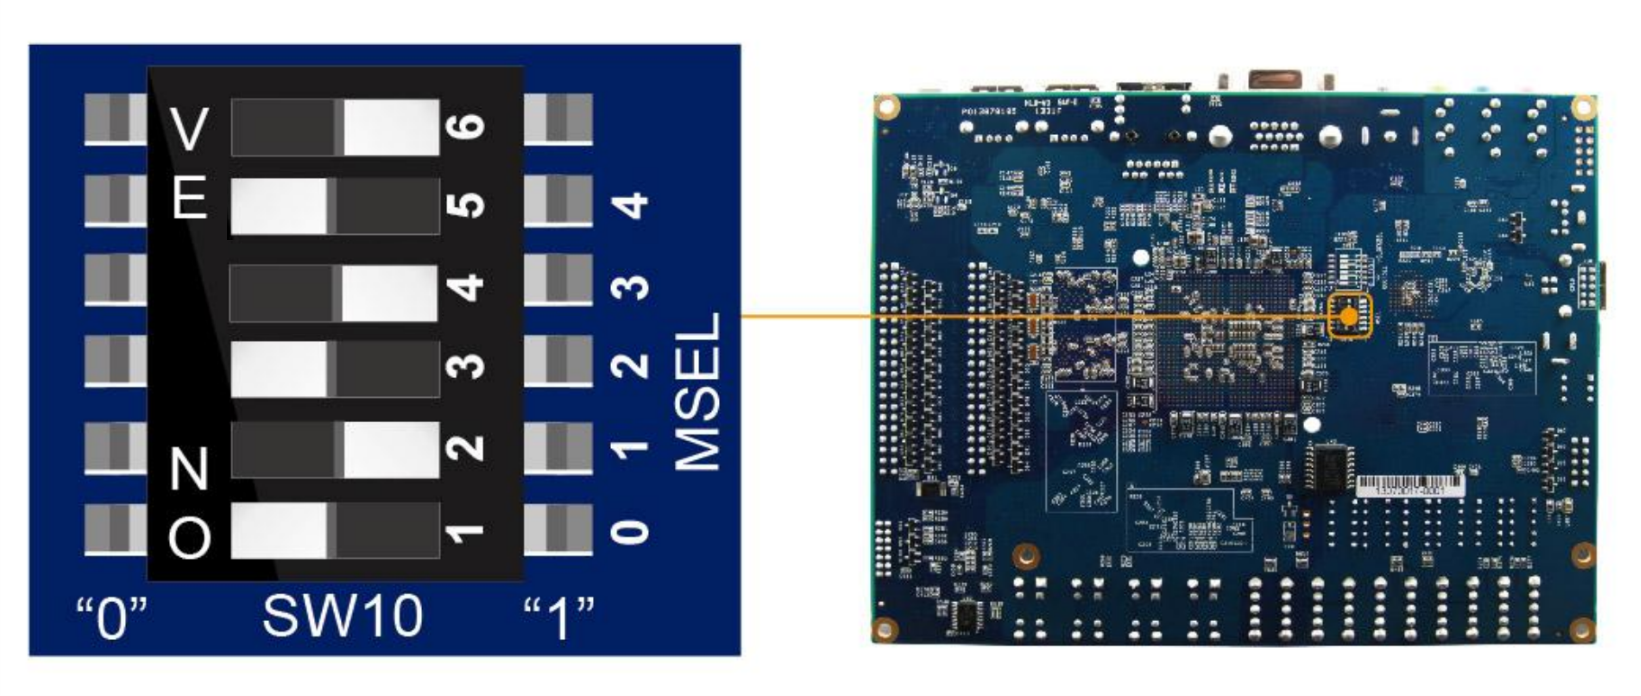
\includegraphics[scale=0.4]{img/de1.png}
\caption{Podešavanje prekidača \texttt{MSEEL} za softversko konfigurisanje FPGA, pozicija prekidača na ploči razvojnog sistema}
\label{slika1:de1}
\end{figure}

Sistem povezati na PC računar USB kablom i otvoriti terminal za komunikaciju.

Nakon uključivanja sistema u terminalu će početi ispisivanje sistemskih obaveštenja koja su uobičajena pri pokretanju sistema. Nakon toga biće zatraženo ime korisnika i lozinka. Po unosu ovih informacija dobija se pristup linuks sistemu. Za učitavanje drajvera koristi se komanda \texttt{insmod}. Nakon učitavanja u folderu \texttt{sys/bus/platform/driver/lddipldrv} se pojavljuju sistemski fajlovi za pristup hardveru. Korišćenjem komande za upis u fajl \texttt{leds} se može upisati vrednost koja će se pojaviti na LE diodama. U primeru na slici \ref{slika1:test1} je upisan broj \texttt{10} (binarno \texttt{1010}) i to je ispisano na LE diodama \ref{slika1:test2}.
\ref{slika1:test1}
\begin{figure}[h]
\centering
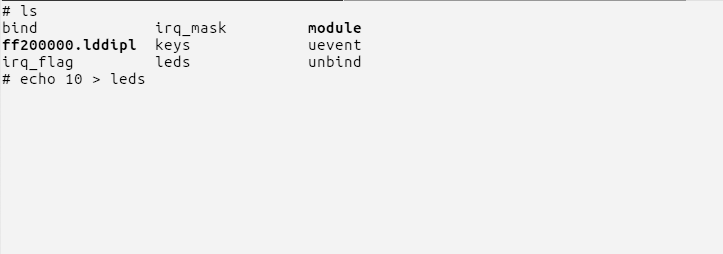
\includegraphics[scale=0.5]{img/test1.png}
\caption{Korišćenje drajvera za uključivanje LE dioda}
\label{slika1:de1}
\end{figure}
\begin{figure}[h]
\centering
\includegraphics[scale=0.1]{img/test2.png}
\caption{Razvojni sistem DE1-SoC povezan za testiranje}
\label{slika1:test2}
\end{figure}
Za demonstraciju pristizanja prekidne rutine je potrebno dozvoliti prekida na tasteru \texttt{1} upisom u sistemski fajl \texttt{irq\_mask}. Nakon pritiskanja tastera na razvojnom sistemu u konzoli se pojavlju obaveštenje koje ispisuje prekidna rutina drajvera \ref{slika1:test3}\\
\begin{figure}[h]
\centering
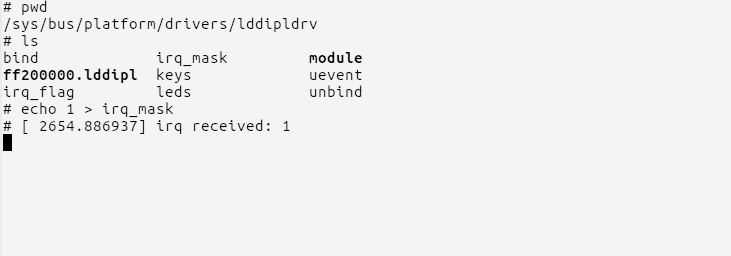
\includegraphics[scale=0.5]{img/test3.png}
\caption{Dozvola prekida i pristizanje prekidne rutine}
\label{slika1:test3}
\end{figure}
Ovim postupcima je pokazan ispravan rad projektovanog sistema. \\
\pagebreak
